\chapter*{Proposition 17}
\label{prop:17}


\begin{figure*}[ht]
    \begin{center}
    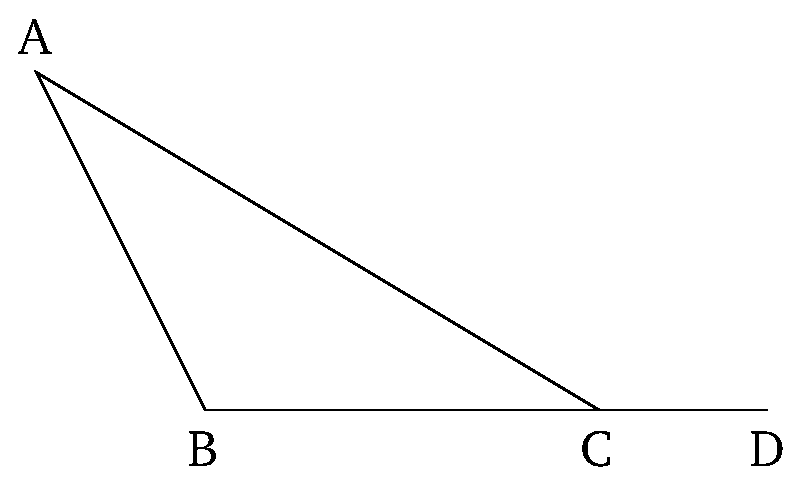
\includegraphics[width=0.5\linewidth]{figures/fig17e.eps}
    \label{fig:prop_17}
    \end{center}
\end{figure*}

For any triangle,  (the sum of) two angles taken together in any (possible way) is less than two right-angles.

Let $ABC$ be a triangle. I say that (the sum of) two angles of triangle $ABC$
taken together in any (possible way) is less than two right-angles.

For let $BC$ have been produced to $D$.

And since the angle $ACD$ is external to triangle $ABC$, it is greater than the
internal and opposite angle $ABC$ [Prop.~1.16]. Let $ACB$ have been added to both. Thus, the
(sum of the angles) $ACD$ and $ACB$ is greater than the  (sum of the angles) $ABC$ and
$BCA$. But, (the sum of) $ACD$ and $ACB$ is equal to two right-angles [Prop.~1.13].
Thus, (the sum of) $ABC$ and $BCA$ is less than two right-angles. Similarly,
we can show that (the sum of) $BAC$ and $ACB$ is also less than two right-angles,
and further (that the sum of) $CAB$ and $ABC$ (is less than two right-angles).

Thus, for any triangle,  (the sum of) two angles taken together in any (possible way) is less than two right-angles. (Which is) the very thing
it was required to show.


\section*{Commentary}

\begin{proposition}\label{proposition_17}\lean{Elements.Book1.proposition_17}\leanok
    In $\triangle~ABC$, we have $\angle~ABC + \angle~BCA$ is less than 180 degrees. 
\end{proposition}
\begin{proof}
    \uses{proposition_13,proposition_16}\leanok
    See the original proof by Euclid.
\end{proof}
